\section{System Design}
\label{sec-design}
We designed an end-to-end network architecture consisting of several identical layers in which:
	Each input image (or each lane from the output of the previous layer) is assigned to its own lane and processed by several convolutional layers. These layers share parameters across channels; however, each image is processed individually and do not interact with each other in this stage. Each channel will present a feature map of n channels.
	The features extracted from all layers are merged broadwise with the following function:


    $${x'_k=\sum x_ie^{kx_i}/\sum e^{kx_i}}$$


Where k varies from -1 to 1. Apparently, k=0 leads to averaging, k=${+\infty}$ leads to a process similar to max operator and k=${-\infty}$ leads to min operator. This process merges information from every lane into one. The output is n channels for each value of k. 
	The original input images are accessed again. These images are also processed separately by several convolutional layers (sharing parameters across lanes) to extract features. The output of these images (m channels each) are stacked with the n channels from step 2) as m+n channels each lane. Some more convolution and an upscaling layer may follow, merging the data more thoroughly. These will be the input for the next layer.
The above 3 steps are stacked as one layer. The functional network often consists of 5 to 8 layers to achieve 4x super resolution. The network ends with a merging process similar to the 2) step and a few more layers of convolution. The full structure of a 3 layer network is shown in Fig~\ref{fig-system}.

\begin{figure}
 \centering
    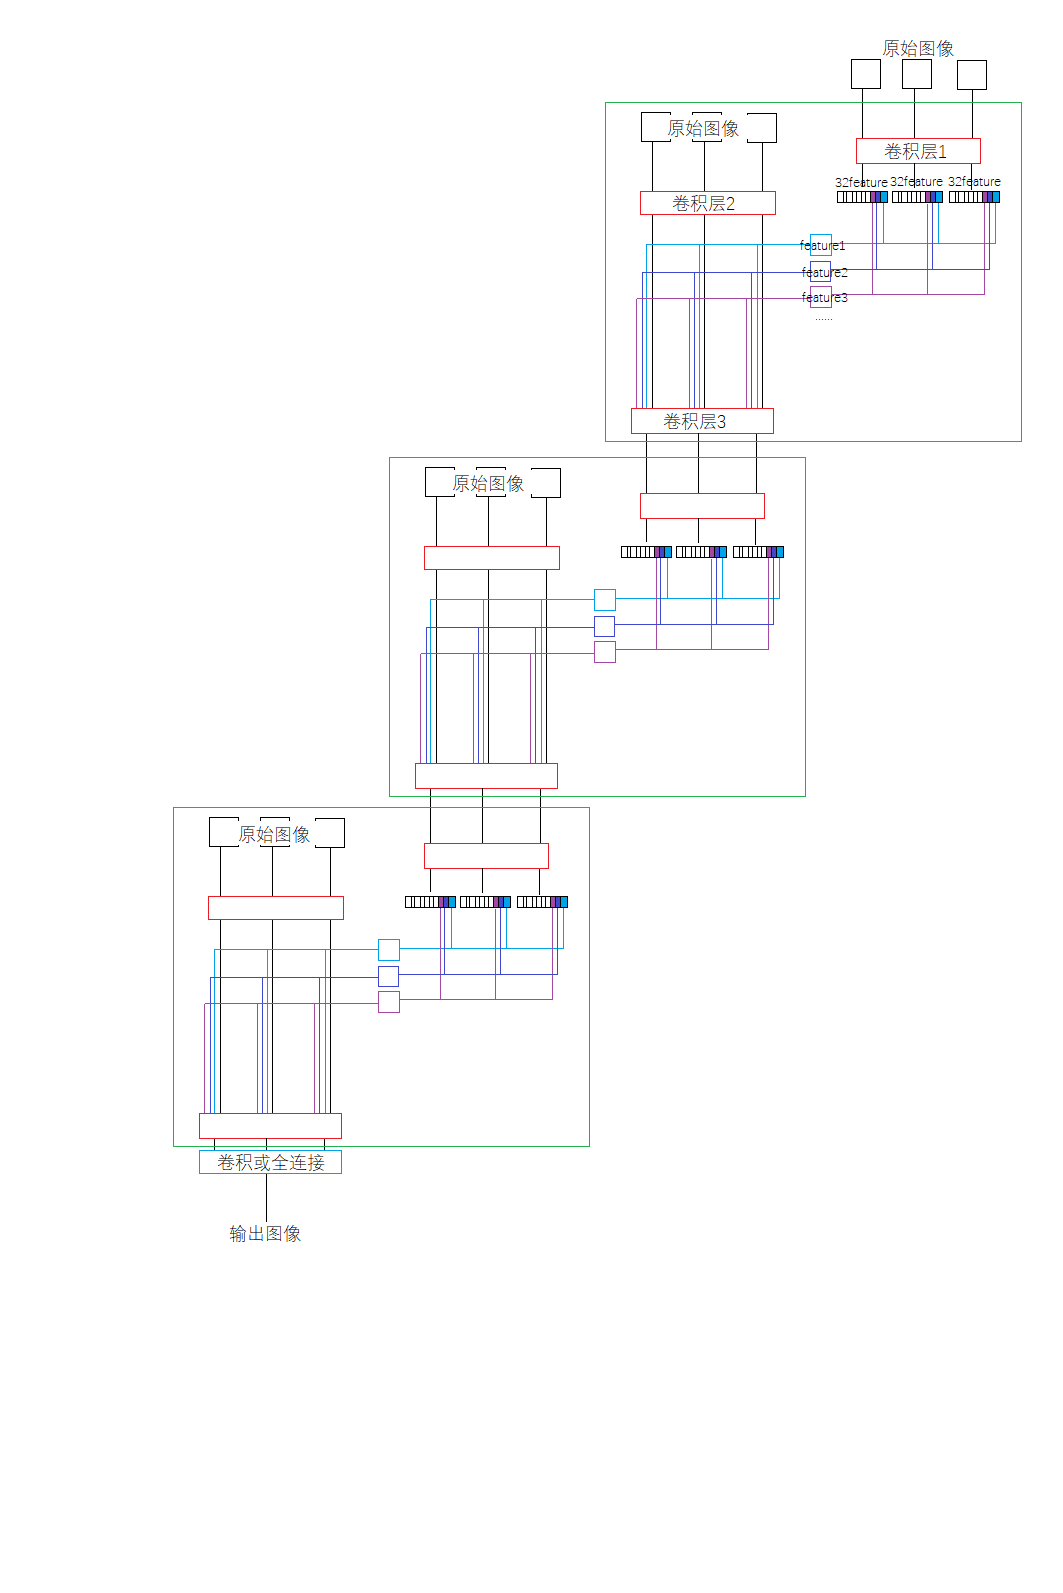
\includegraphics[width=0.375\textwidth]{./pic/system}
    \caption{Network Architecture of SRPeek.}
    \label{fig-system}
\end{figure}
